\newpage
\subsection{Utilizzo dell'applicativo}
Alla fine della fase di codifica, assistito dal tutor, ho creato gli eseguibili (installers oppure pacchetti, a seconda della piattaforma), attraverso Electron Forge.\\
Allo stato da me raggiunto, ENGaming può essere utilizzato con:
\begin{itemize}
    \item un PC con installato il driver \gls{displaylink} e uno dei seguenti sistemi operativi: \begin{itemize}
    \item Windows 11 (non necessario installare il driver citato in precedenza, in quanto già presente).
    \item MacOS Ventura.
    \end{itemize}
    \item un ENSign11 da collegare a suddetto PC.
\end{itemize}
Purtroppo non ho potuto testare l'applicativo in altre versioni di Windows o MacOS, a causa della mancanza di tempo nel farlo. Non sono invece stati testati altri device di firma poichè non sono stati considerati come device target, a differenza dell'ENSign11.\\
Su sistemi operativi con kernel Linux, l'applicativo veniva eseguito ma non riconosceva il tablet, costringendo un utilizzo tramite tastiera e mouse e in generale con errori dovuti proprio al non riconoscimento del device.
\newpage
\subsection{Panoramica del prodotto}
Per concludere questa sezione, voglio mostrare il frutto della fase di codifica, partendo dalla schermata iniziale e concludendo con la gestione dell'inattività.\\
\subsubsection{Parti prodotte}
La schermata iniziale dell'applicazione comprende:
\begin{itemize}
    \item Il nome dell'applicazione stessa.
    \item L'elenco dei giochi disponibili, sotto forma di icone.
    \item Un'icona per visualizzare i record effettuati.
    \item Un'icona per uscire dall'applicazione.
\end{itemize}
\begin{figure}[h]
    \centering
    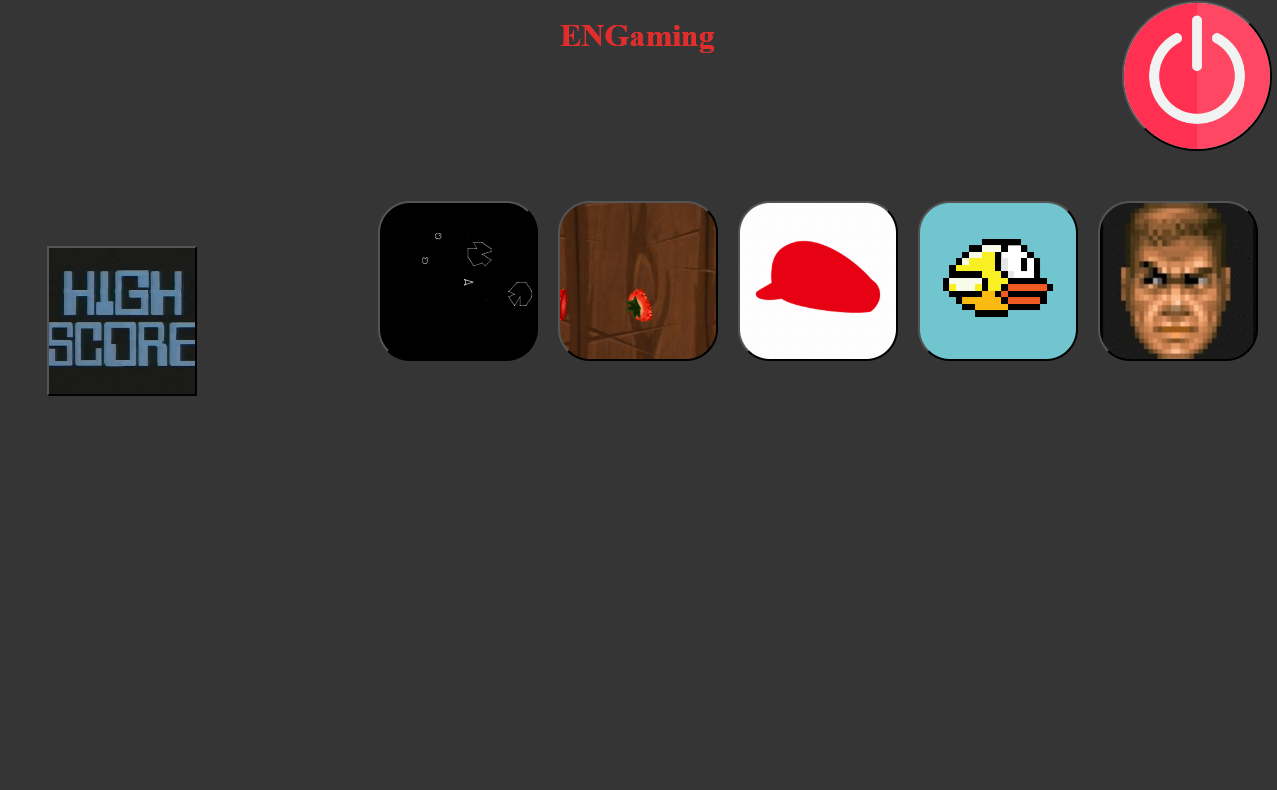
\includegraphics[width=250pt]{images/product/schermataIniziale.png}
    \caption{Schermata iniziale di ENGaming}
    \label{fig:schermataIniziale}
\end{figure}
Ho scelto una visualizzazione il più possibile vicina alle icone per portare un senso di famigliarità, in quanto ENGaming viene usato attraverso uno schermo touch.
\newpage
Atraverso l'icona "High Score", è possibile passare alla visualizzazione dei record.\\
La pagina apposita mostra la lista dei record globale, ovvero mostra tutti i record effettuati senza distinzione di gioco.\\
In particolare, ogni record mostra:
\begin{itemize}
    \item l'utente che ha effettuato il record
    \item il punteggio totalizzato
    \item la data in cui è stato effettuato il record
    \item il gioco in cui è stato effettuato il record
\end{itemize}
\begin{figure}[h]
    \centering
    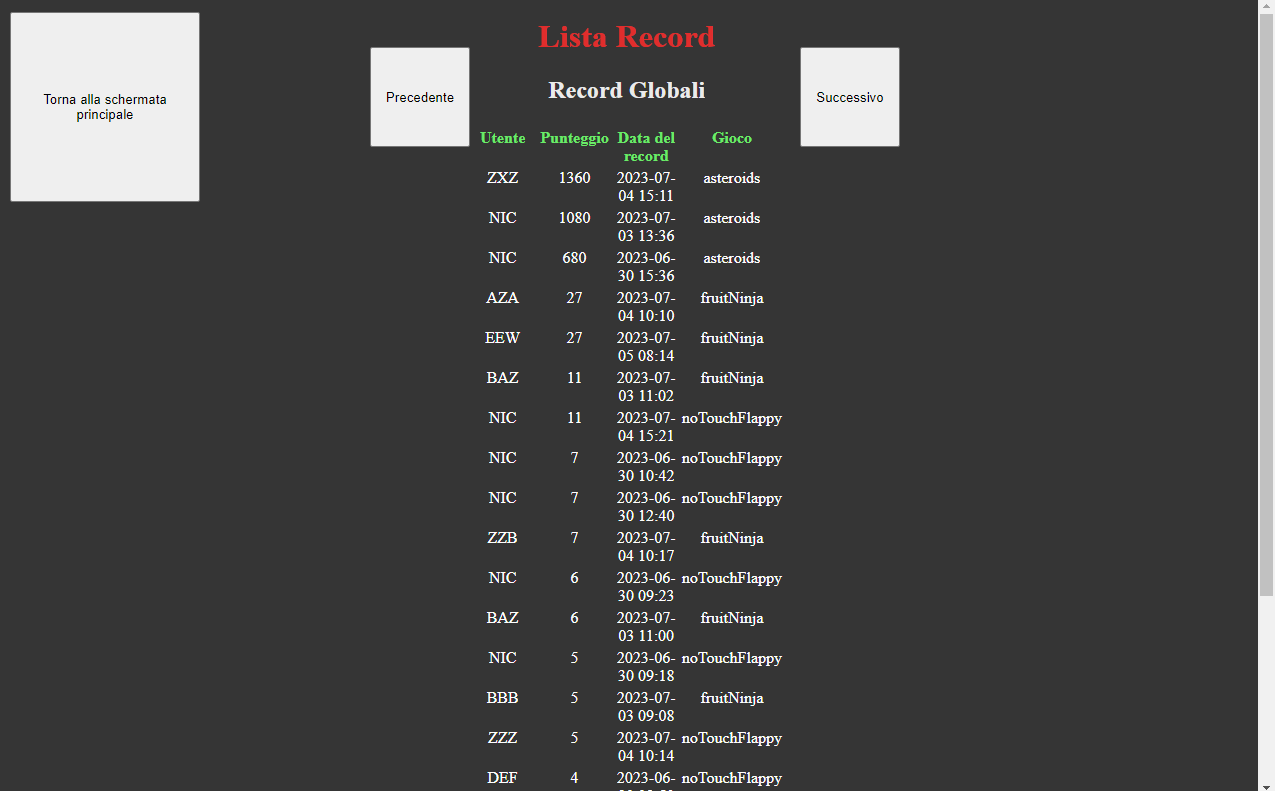
\includegraphics[width=250pt]{images/product/schermataRecord.png}
    \caption{Lista dei record globali}
    \label{fig:schermataRecord}
\end{figure}
Utilizzando i pulsanti "attorno" alla lista, si può passare alla lista dei record per i giochi specifici.\\
Tali liste sono tante quanti i giochi in cui sia stato fatto almeno un record.
La prima e l'ultima lista di questo genere, alla pressione degli appositi pulsante, riportano alla lista globale.
\begin{figure}[h]
    \centering
    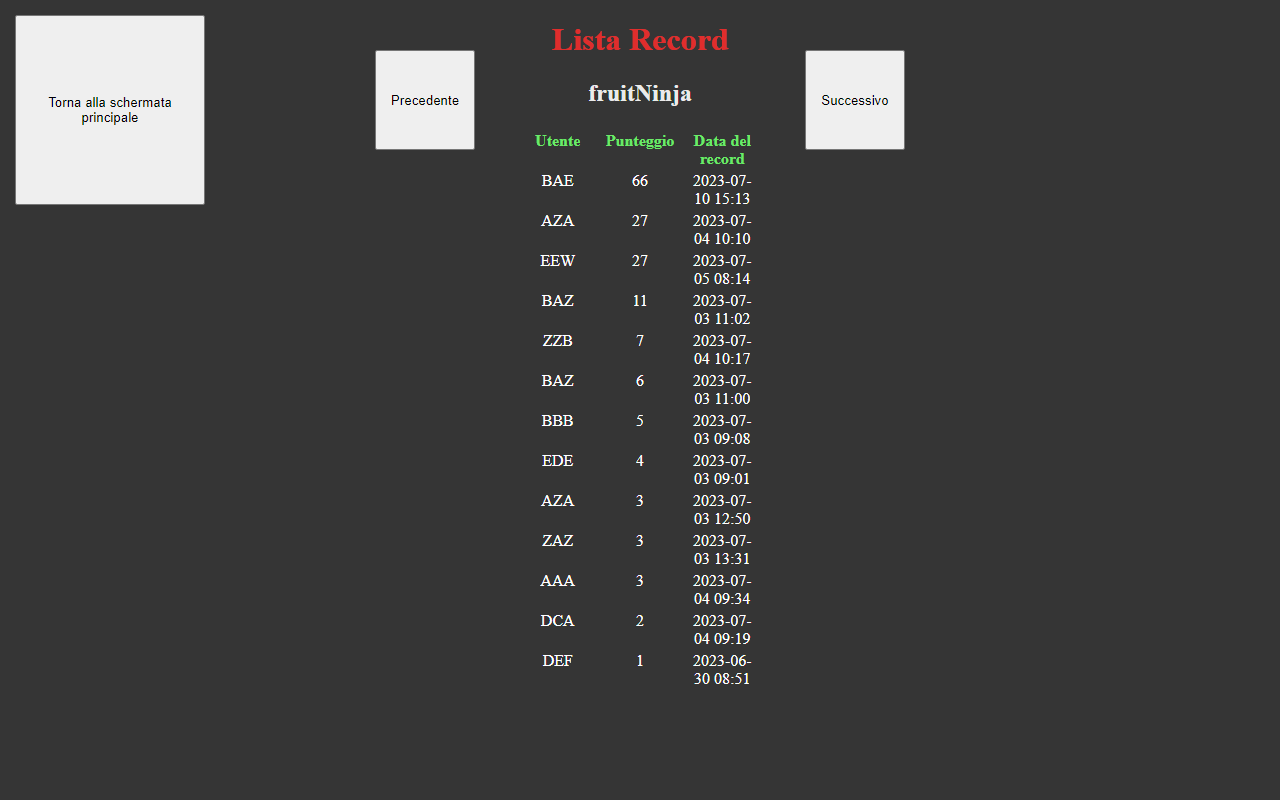
\includegraphics[width=250pt]{images/product/schermataRecordSingoloGioco.png}
    \caption{Esempio di lista per un singolo gioco}
    \label{fig:schermataRecordSingoloGioco}
\end{figure}
\newpage
Ritornando alla schermata iniziale, si può selezionare un gioco attraverso la propria icona.\\
Tale operazione porta alla pagina del gioco stesso, che contiene le informazioni sul gioco stesso, ovvero:
\begin{itemize}
    \item il nome del gioco.
    \item il genere del gioco.
    \item il tipo di input, ovvero se viene utilizzato il controller o il touch/digitalizer.
    \item la descrizione del gioco.
    \item L'elenco degli input, o delle gesture, che il gioco ha.
\end{itemize}
\begin{figure}[h]
    \centering
    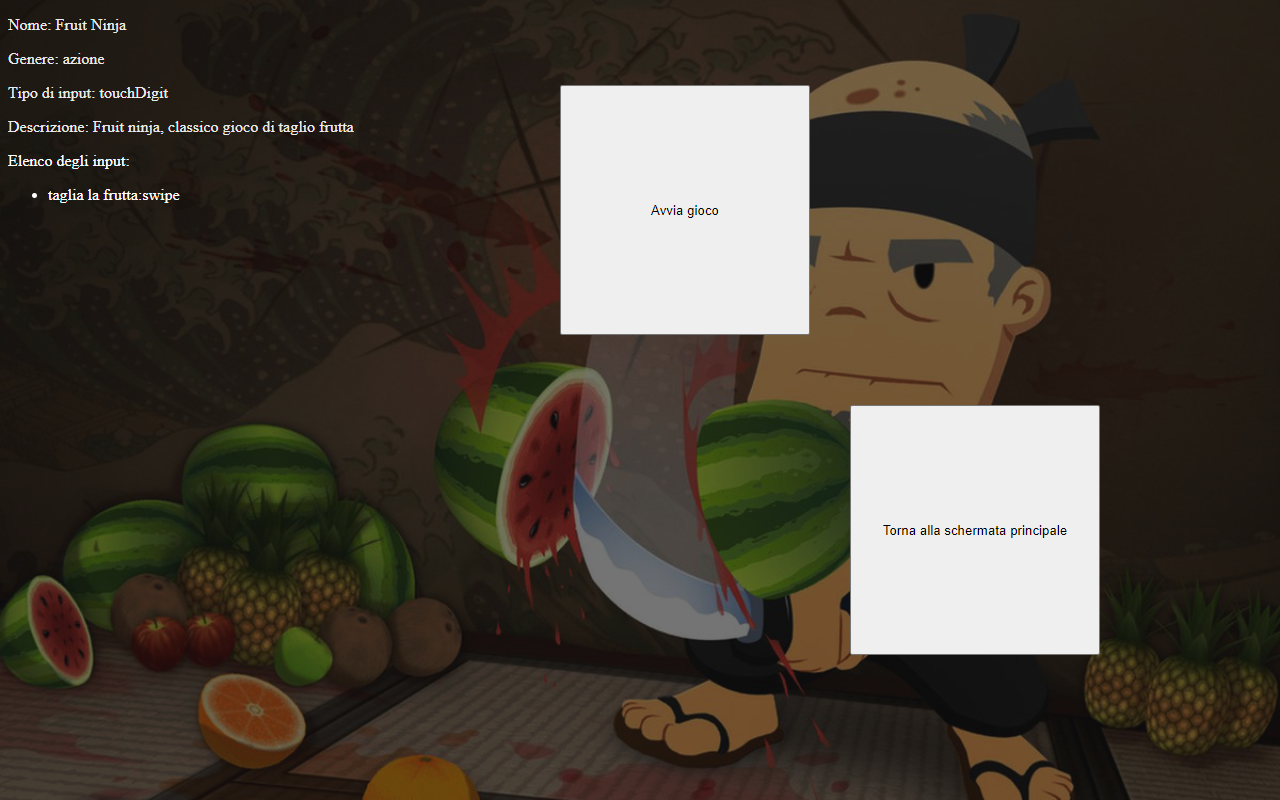
\includegraphics[width=250pt]{images/product/schermataPaginaGioco.png}
    \caption{Esempio di pagina di un gioco}
    \label{fig:schermataPaginaGioco}
\end{figure}
Ovviamente, da questa pagina si può decidere se avviare il gioco o tornare alla schermata principale.\\\\
All'avvio del gioco, si passa attraverso una pagina di caricamento. La pagina in questione è spoglia, in quanto informa semplicemente l'utente dello stato di caricamento.\\
Questa pagina viene visualizzata per 4 secondi, per poi passare all'interfaccia di gioco.
\begin{figure}[h]
    \centering
    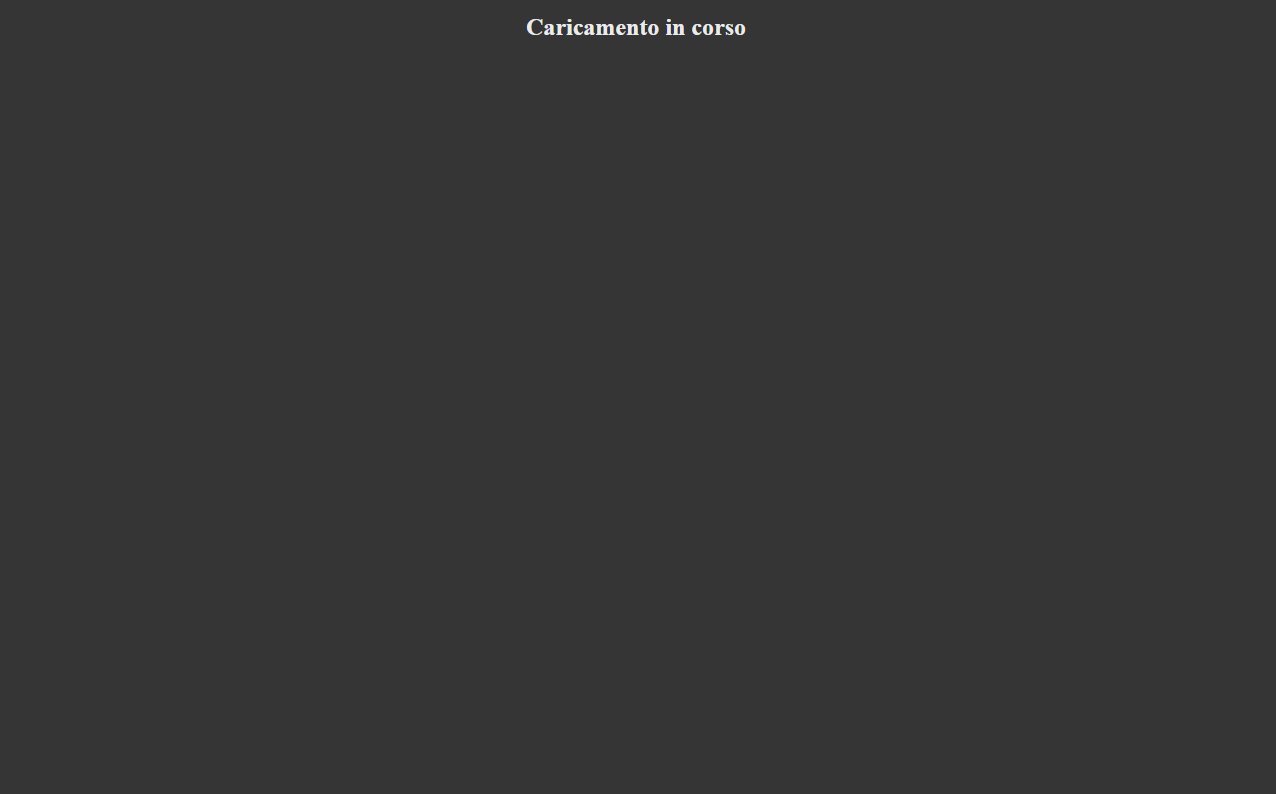
\includegraphics[width=250pt]{images/product/schermataCaricamento.png}
    \caption{Schermata di caricamento}
    \label{fig:schermataCaricamento}
\end{figure}
\newpage
La differenza tra le due tipologie di gioco entra adesso.\\
Infatti, se il gioco prevede l'utilizzo del controller, oltre al gioco stesso si visualizza anche il controller, che dalla struttura di default (spiegata in \nameref{paragraph:gamecontrollerinterfacecomponent}), viene configurato attraverso gli input che il gioco richiede.
\begin{figure}[h]
    \centering
    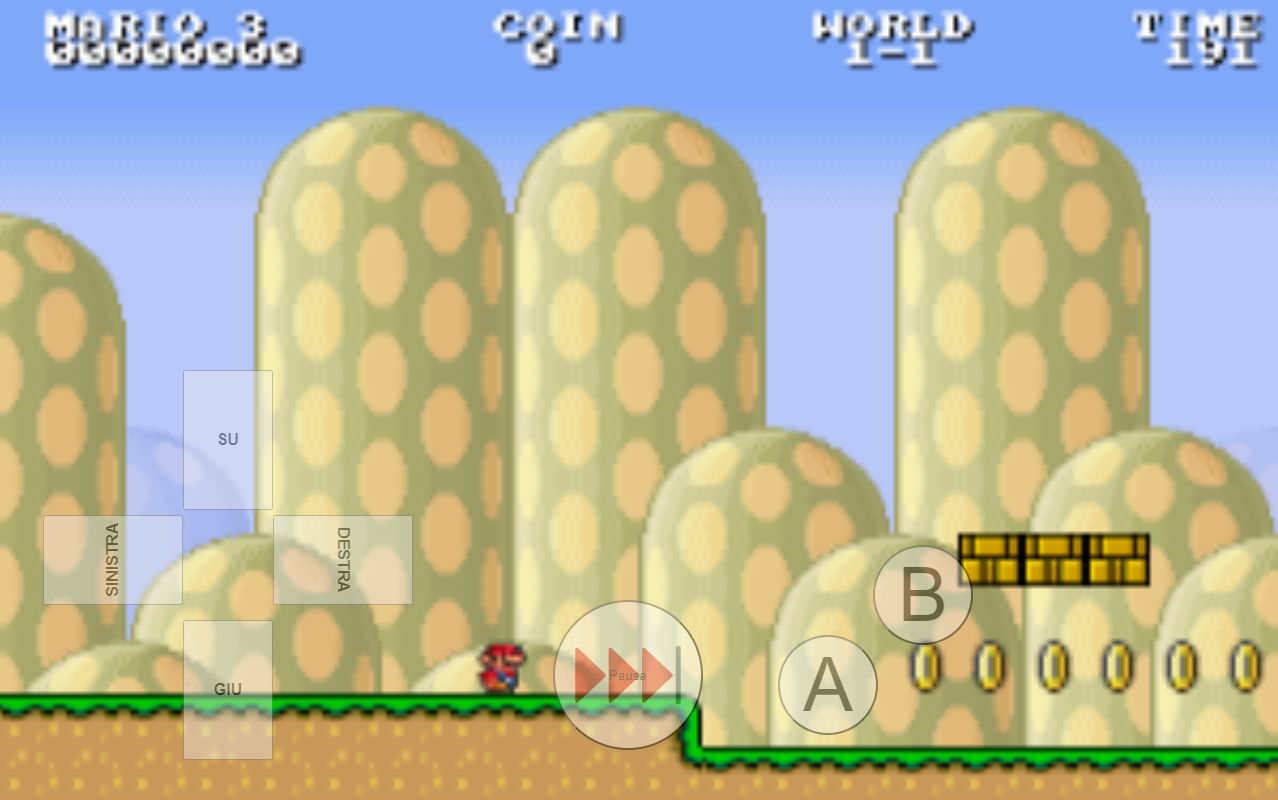
\includegraphics[width=250pt]{images/product/schermataGiocoController.png}
    \caption{Esempio di schermata per un gioco con il controller}
    \label{fig:schermataGiocoController}
\end{figure}
\newpage
Mentre, se il gioco prevede l'utilizzo del touch o del digitalizer, ciò che viene visualizzato sono solo il gioco e il pulsante di pausa, essendo gli input del gioco dati dalle gestures.\\
\begin{figure}[h]
    \centering
    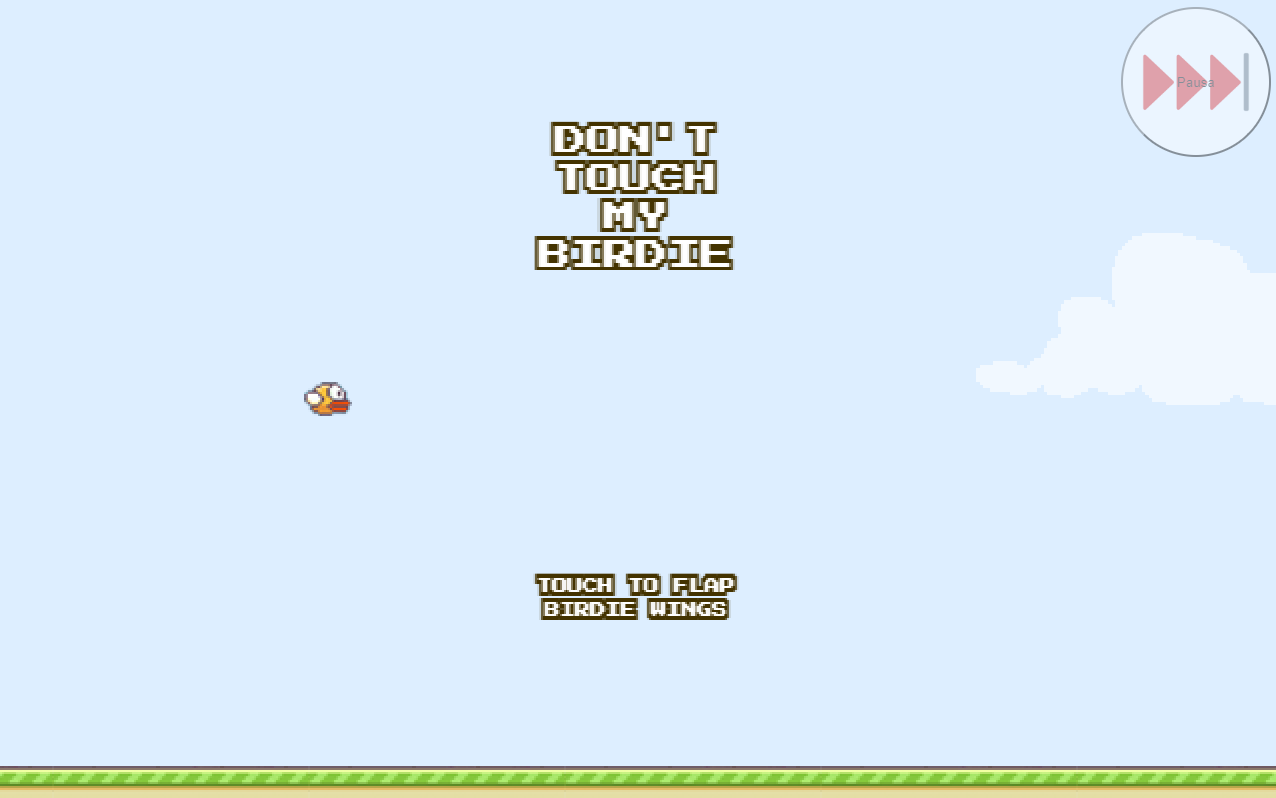
\includegraphics[width=250pt]{images/product/schermataGiocoTouchDigit.png}
    \caption{Esempio di schermata per un gioco con il touch/digitalizer}
    \label{fig:schermataGiocoTouchDigit}
\end{figure}
\\
In ogni gioco, a prescindere dal tipo, premendo sul pulsante di pausa si va all'apposita schermata di pausa.\\
La schermata di pausa informa l'utente dello stato di pausa del gioco, e ne permette la ripresa oppure l'uscita dallo stesso.
\begin{figure}[h]
    \centering
    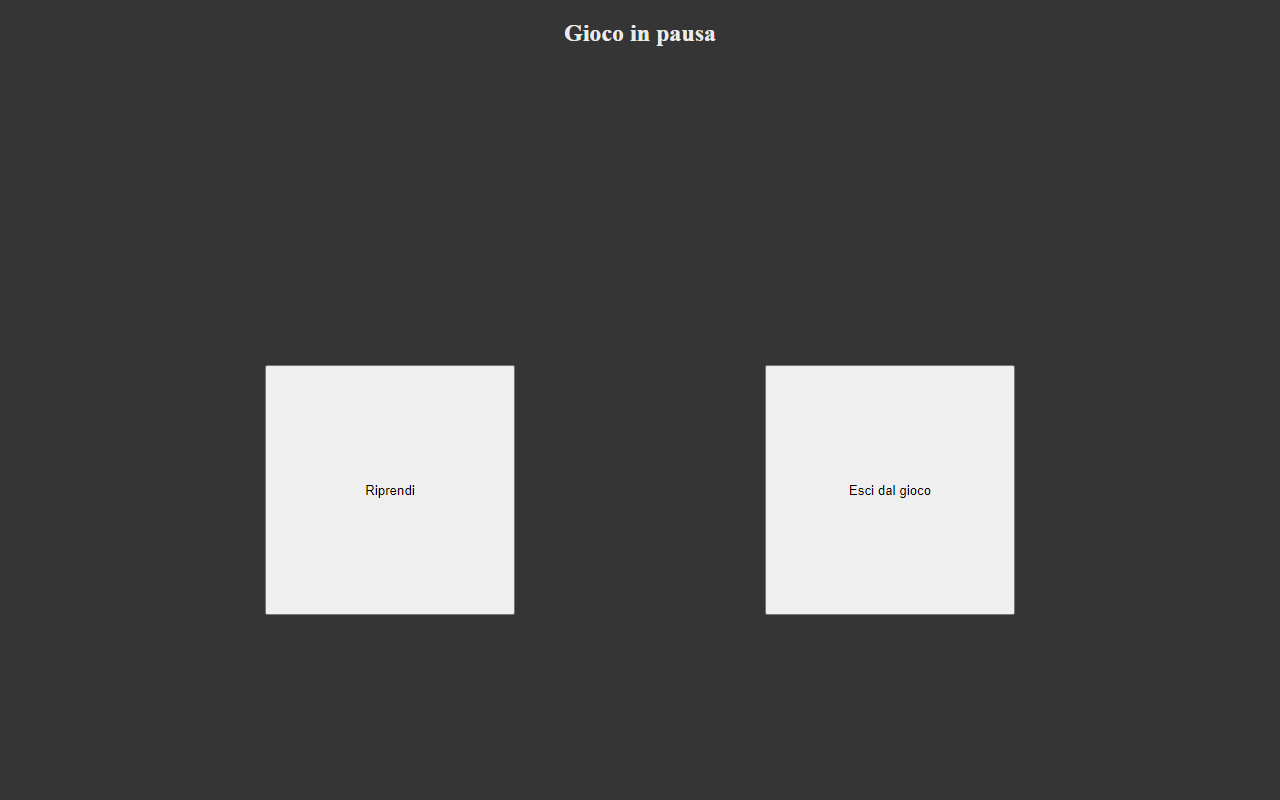
\includegraphics[width=250pt]{images/product/schermataPausaGioco.png}
    \caption{Schermata di pausa}
    \label{fig:schermataPausaGioco}
\end{figure}
\newpage
Ovviamente una parte importante dell'applicazione è il salvataggio dei record effettuati nei giochi. Per far questo, si passa attraverso due schermate.\\
La prima informa semplicemente l'utente che ha effettuato un nuovo record nel gioco appena concluso. Olte a questo, permette allo stesso di decidere se salvarlo o meno.\\
\begin{figure}[h]
    \centering
    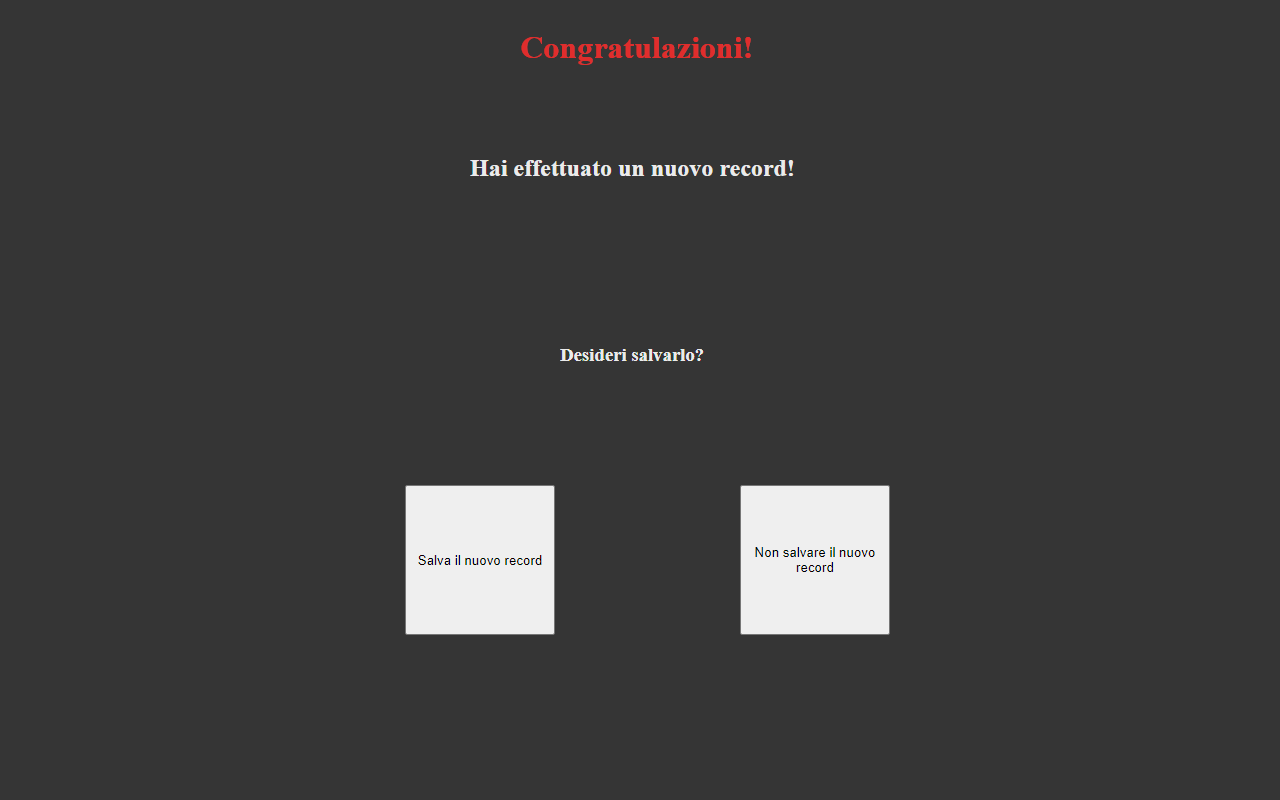
\includegraphics[width=250pt]{images/product/schermataNuovoRecord.png}
    \caption{Schermata di avviso per un nuovo record}
    \label{fig:schermataNuovoRecord}
\end{figure}
\\Nel caso non si voglia salvare il record, l'applicativo semplicemente ritorna nel menù principale, perdendo il punteggio da salvare.\\
Se invece l'utente vuole salvare il record, viene portato alla seconda schermata, dedicata all'inserimento del nome.\\
Il nome viene inserito attraverso dei pulsanti, che permettono di selezionare, una per volta, le tre lettere che compongono il nome a cui associare il record.
\begin{figure}[h]
    \centering
    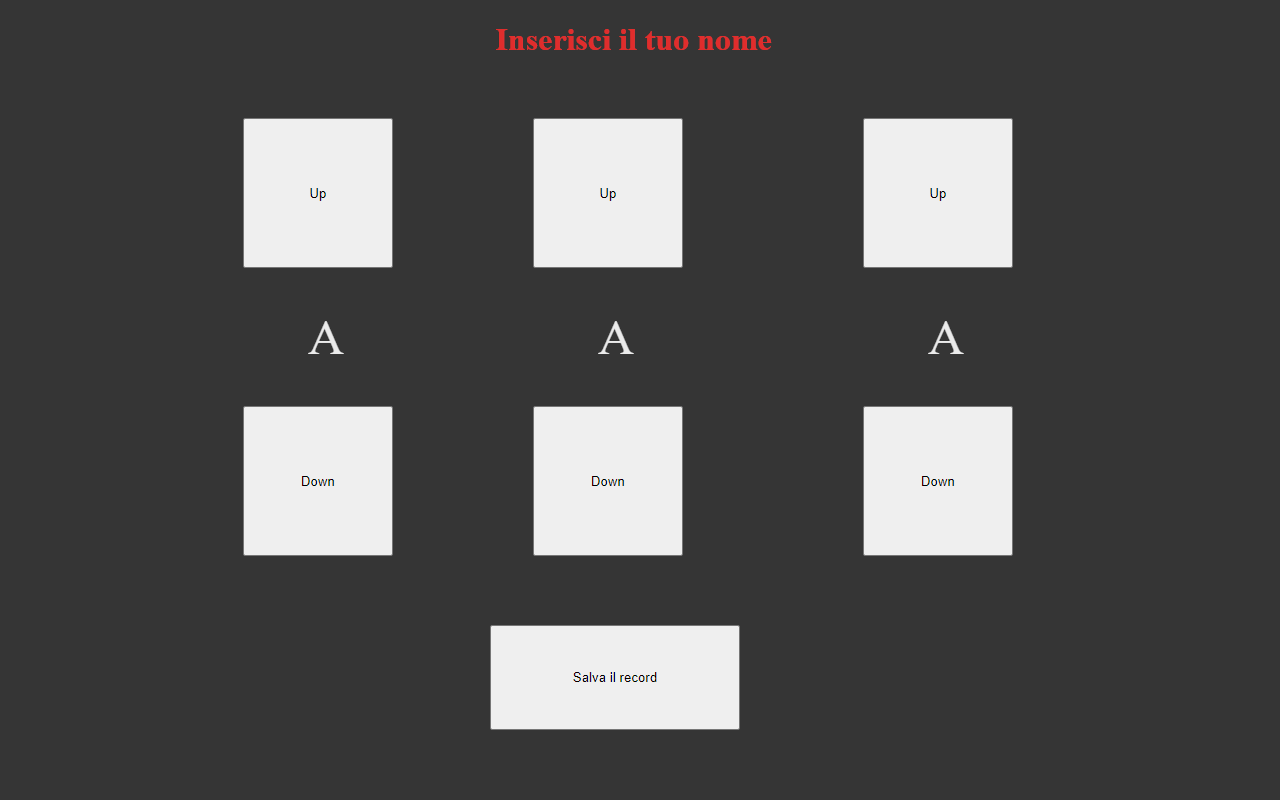
\includegraphics[width=250pt]{images/product/schermataInserimentoNome.png}
    \caption{Schermata per l'inserimento del nome}
    \label{fig:schermataInserimentoNome}
\end{figure}
\\Ho scelto lo stile dei giochi arcade per un principio specifico, ovvero l'inserimento di input senza dover ricorrere a periferiche esterne a quelle presenti. Infatti, grazie a questa modalità, si può utilizzare lo schermo del device senza incorre in tastiere virtuali o fisiche.
\subsection{Gestione degli errori}
A livello di comportamento, ENGaming prevede pochi casi di errore, essendo un sistema che non prevede configurazioni da parte dell'utente.\\
Voglio comunque elencare delle piccole accortezze che ho implementato, in quanto si sono rivelate utili anche alla prevenzione di altri errori.
\subsubsection{Gestione del non collegamento del device}
ENGaming, durante l'avvio, cerca di individuare un ENSign11, in modo da collocarci l'applicazione al suo interno. Nel caso l'utente non colleghi un device prima dell'avvio, l'applicazione riporta un errore all'utente, terminando l'esecuzione del programma.
\subsubsection{Gestione dell'inattività}
\label{sec:inactivity}
L'applicazione, se non rileva alcun input per 10 secondi, fa partire un timer di inattività della durata massima di 4 minuti. Tale timer si azzera se durante questo lasso di tempo riceve un input.\\
Nel caso scada il tempo, il sistema chiude l'attività in esecuzione (gioco o salvataggio del record) e ritorna alla schermata principale.\\
Tale azione comporta la perdita di un eventuale record effettuato e non ancora salvato, in quanto l'attività precedentemente in esecuzione viene chiusa forzatamente.